\documentclass{standalone}
\usepackage{tikz}
\begin{document}
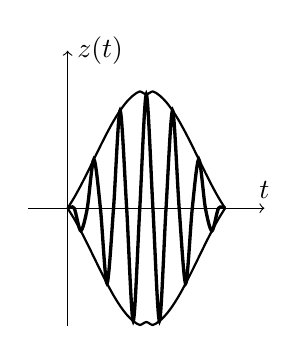
\begin{tikzpicture}[scale=2]
    \draw[->](-0.25,0)--(1.25,0)node[above]{$t$};
    \draw[->](0,-0.75)--(0,1)node[right]{$z(t)$};
    
    \draw[very thick,smooth, domain=0:1]plot(\x,{0.75*cos(12*pi*\x r)*sin(2*pi*(\x-0.5) r)/(2*pi*(\x-0.5))});
    \draw[thick,,smooth, domain=0:1]plot(\x,{0.75*sin(2*pi*(\x-0.5) r)/(2*pi*(\x-0.5))});
    \draw[thick,,smooth, domain=0:1]plot(\x,{-0.75*sin(2*pi*(\x-0.5) r)/(2*pi*(\x-0.5))});
\end{tikzpicture}
\end{document}